\chapter{Технические методы}
\begin{important}
Не стоит забывать, что следующие методы необходимо использовать, по возможности, совместно друг с другом и с методами, перечисленными в предыдущей главе.
\end{important}

\section{Прокси}
\begin{important}
Не забывайте, что хозяева прокси-серверов и анонимайзеров видят трафик нешифрованным.
\end{important}
\begin{important}
Некоторые прокси-сервера передают заголовок X-Forwarded-For с реальным IP-адресом клиента.
\end{important}
\textbf{Прокси-сервер} --- сервер, который позволяет пропускать через себя пользовательский трафик.\\
Для использования прокси просто задайте его адрес в настройках браузера и других приложений, трафик которых вы хотите пропускать через прокси.
\subsection{Списки открытых прокси}
\begin{enumerate}
\item \url{http://xroxy.com}
\item \url{https://hidemyass.com/proxy-list}
\item \url{http://freeproxy.ch}
\item \url{http://proxylists.net}
\item \url{http://nntime.com}
\end{enumerate}

\section{Веб-прокси}
\textbf{Веб-прокси}) --- веб-страница, которая позволяет пользователю получить контент с заданного адреса через себя.\\
Для использования веб-прокси, перейдите на его страницу и введите адрес сайта, который вы хотете посетить.
\subsection{Некоторые веб-прокси}
\begin{enumerate}
\item \url{https://hidemyass.com}
\item \url{http://anonymouse.org}
\item \url{http://hide.pl}
\item \url{http://hideme.ru}
\item \url{http://guardster.com/free/}
\end{enumerate}

\section{VPN}
\begin{important}
Не забывайте, что хозяин VPN-сервиса видит трафик нешифрованным.
\end{important}
\textbf{VPN} --- технология, позволяющая создавать сети поверх существующего Интернет-подключения. Из-за высокой скорости работы, простоты настройки и шифрования трафика от клиента до VPN-провайдера часто используется как средство сокрытия реального IP-адреса при доступе в Интернет. VPN-провайдеры обычно предоставляют свои услуги на платной основе.
\subsection{Некоторые VPN-провайдеры}
\begin{enumerate}
\item \url{https://ipredator.se}
\item \url{https://kebrum.com}
\item \url{https://relakks.com}
\item \url{https://vpntunnel.se}
\item \url{http://ivacy.com}
\end{enumerate}

\section{SSH-туннели}
\textbf{SSH} --- протокол, созданный для безопасной передачи данных. Часто используется для удаленного управления другими компьютерами, но может использоваться и для создания туннелей.\\
\textbf{SSH-туннель} --- туннель, созданный с помощью SSH-соединения и используемый для передачи данных. Существуют организации, предоставляющие SSH-туннелирование на платной основе.
\subsection{Использование}
\begin{lstlisting}
ssh -D localhost:port login@address
\end{lstlisting}
port --- порт, трафик на который будет пропускаться через SSH-туннель.\\
login --- ваш логин на удаленном сервере.\\
address --- адрес удаленного сервера.\\
После этого установите в приложениях, трафик которых вы хотите туннелировать, например, в браузере, адрес SOCKS-прокси localhost с портом, который вы указали в предыдущем шаге.
\subsection{Некоторые провайдеры SSH-туннелей}
\begin{enumerate}
\item \url{https://tunnelr.com}
\item \url{http://torvpn.com}
\item \url{http://vpnsecure.me}
\item \url{http://guardster.com}
\item \url{http://anonyproz.com}
\end{enumerate}

\section{Настройка браузера}
\begin{important}
Браузер передает огромное количество информации. По отдельности эта информация не представляет никакого интереса, но собранная вместе она может позволить практически со 100\% вероятностью установить вашу личность.
\end{important}
\subsection{Настройка браузера Firefox}
Для изменения настроек можно использовать специальную страницу \textit{about:config} или добавлять их напрямую в файл настроек \textit{prefs.js}, находящийся в папке профиля. Некоторые полезные настройки доступны через стандартное меню настроек
\subsubsection{Предпочитаемые языки}
В меню <<Настройки>> \textrightarrow <<Содержимое>> \textrightarrow <<Языки>> удалите из списка все языки, кроме английского. Порядок должен быть en-us, затем en. Несмотря на то, что многие сайты будут теперь использовать по умолчанию английский язык, это повысит вашу анонимность, так ваш браузер станет менее уникальным.
\subsubsection{Шрифты}
По умолчанию Firefox передает список установленных шрифтов. Это может повысить уникальность вашего браузера, что отрицательно скажется на анонимности. Для отключения этого в \textit{about:config} нужно поменять значение \textit{browser.display.use\_document\_fonts} на 0.
\subsubsection{Local storage}
По умолчанию в Firefox включен Local storage и браузеру присвоен уникальный ID. Также страницы могут записывать в него свою информацию. Отключить Local storage можно изменением в \textit{about:config} значения \textit{dom.storage.enabled} на \textit{false}.
\subsubsection{Кеш}
Для того, чтобы скрыть факт повторного посещения страницы, необходимо отключить кеш. Измените в \textit{about:config} значения \textit{browser.cache.disk.enable} и \textit{browser.cache.memory.enable} на \textit{false}.
\subsubsection{DNS-запросы через SOCKS5 прокси}
По умолчанию Firefox делает DNS-запросы в обход SOCKS5-прокси (например, при использовании Tor), что может помочь установить провайдеру, какие сайты вы посещали. Измените значение \textit{network.proxy.socks\_remote\_dns} на \textit{true}.
\subsubsection{Передача информации о посещенных сайтах}
Установите значение \textit{browser.safebrowsing.enabled} в \textit{false} и \textit{browser.safebrowsing.malware.enabled} в \textit{false} для тключения передачи информации о посещаемых веб-сайтах (система для борьбы с фишингом).
\subsubsection{Подмена User Agent}
Заменить значение User Agent можно и без расширений. Для этого существует параметр \textit{general.useragent.override}, установите его значение, например, в  \textit{<<Mozilla/5.0 (Windows; U; Windows NT 5.1; en-US; rv:1.9.1.7) Gecko/200091221 Firefox/3.5.7>>}. Если выставить наиболее распространённое значение, то это поможет снизить уникальность пользователя.
\subsubsection{Запрет Cookie для сторонних сайтов}
Установите значение \textit{network.cookie.cookieBehavior} в 1 для запрета Cookies для сторонних сайтов.
\subsubsection{Запрет на передачу заголовка HTTP referer}
Установите значение item \textit{network.http.sendRefererHeader} в  0 для отключения передачи заголовка HTTP referer для обычного соединения, и значение  \textit{network.http.sendSecureXSiteReferrer} в 0 для отключения передачи для зашифрованного соединения.
\subsubsection{Отключение Java}
Для отключения Java установите значение \textit{security.enable\_java} в \textit{false}.
\subsection{Дополнения}
\subsubsection{HTTPS Everywhere}
HTTPS Everywhere --- дополнение для браузеров Firefox и Chrome/Chromium, переадресующее на HTTPS версию сайта, если она доступна. Это позволяет защититься от перехвата передаваемых данных, но не позволяет скрыть сам факт посещения вебсайта. Скачать дополнение можно тут \url{https://eff.org/https-everywhere}.
\subsubsection{BetterPrivacy}
BetterPrivacy --- дополнение для браузера Firefox, позволяющее удалять флеш-куки (Local Shared Objects). Это небольшие куски данных, которые Adobe Flash может сохранять на компьютерах. Ссылка: \url{https://addons.mozilla.org/firefox/addon/betterprivacy/}.
\subsubsection{Ghostery}
Ghostery --- дополнение для браузеров Firefox, Safari, Chrome/Chromium, Opera и Internet Explorer, позволяющее блокировать скрипты, невидимые изображения и прочие методы, используемые многими компаниями для слежки за пользователями. Работает и с LSO, может заменить BetterPrivacy. Сайт: \url{https://www.ghostery.com}.
\subsubsection{TrackerBlock}
TrackerBlock --- дополнение, аналогичное по функционалу Ghostery, доступное для браузеров Firefox, Chrome/Chromium и Internet Explorer. Сайт: \url{http://privacychoice.org/trackerblock}.
\subsubsection{Beef Taco}
Beef Taco --- дополнение для браузера Firefox, позволяющее блокировать куки ресурсов, шпионящих за пользователями. Сайт: \url{http://jmhobbs.github.com/beef-taco/}.
\subsubsection{User Agent Switcher}
User Agent Switcher --- дополнение для браузера Firefox, позволяющее менять заголовок User-Agent, передаваемый браузером. Сайт: \url{http://chrispederick.com/work/user-agent-switcher/}. Вы можете скачать дополнительный список User-Agent здесь \url{http://techpatterns.com/forums/about304.html} и импортировать его в дополнение.
\subsubsection{Smart Referer}
Smart Referer --- дополнение для браузера Firefox, которое позволяет отправлять адрес предыдущей страницы только если она находится на этом же домене. Скачать: \url{https://addons.mozilla.org/firefox/addon/smart-referer/}.
\subsubsection{TrackMeNot}
TrackMeNot --- дополнение для браузеров Firefox и Chrome/Chromium, делающее переодические поисковые запросы к популярным поисковым системам с целью обезличить логи. Сами запросы являются случайными словами из заданной RSS-ленты. Сайт: \url{https://cs.nyu.edu/trackmenot/}.
\subsubsection{NoScript}
NoScript --- дополнение для браузера Firefox, позволяющее блокировать JavaScript, Flash, Java и другие элементы на недоверенных сайтах. Сайт: \url{http://noscript.net}.
\subsubsection{RequestPolicy}
RequestPolicy --- дополнение для браузера Firefox, позволяющее защититься от подделки межсайтовых запросов. Сайт: \url{https://requestpolicy.com}.
\subsubsection{Cookie Monster}
Cookie Monster --- дополнение для Firefox, позволяющее управлять разрешениями на использование Cookies, например, разрешать их использование только доверенным сайтам. Скачать: \url{https://addons.mozilla.org/firefox/addon/cookie-monster/}.
\subsubsection{ipFlood}
ipFlood --- дополнение для Firefox, симулирующее использование прокси путем добавления случайных IP-адресов в заголовки X-Forwarded-For, Client-IP и Via. Скачать: \url{https://addons.mozilla.org/firefox/addon/ipflood/}.
\subsubsection{IPFuck}
IPFuck --- дополнение для Firefox, аналогичное ipFlood. Сайт: \url{http://ipfuck.paulds.fr/}.
\subsection{Плагины}
Сам факт наличия каких-либо редкоиспользуемых плагинов увеличивает уникальность вашего браузера. Также некоторые плагины, например Java, передают ваш настоящий IP адрес, даже если вы за прокси.

\section{Анонимные оверлейные сети}
\begin{important}
Никогда не используйте анонимные сети с настройками, которые позволяют использовать Интернет в одном браузере в обход самой сети. В этом случае будет достаточно вставить любое изображение из внешнего Интернета, чтобы получить ваш реальный IP-адрес.
\end{important}
\textbf{Оверлейные сети} --- это такие сети, которые работают поверх другой уже работающей сети.
\subsection{Tor}
\begin{wrapfigure}[9]{r}{0.25\linewidth}

\includegraphics[width=\linewidth]{Tor}
\caption{Логотип Tor}
\end{wrapfigure}
\textbf{Tor} --- анонимная оверлейная сеть, использующая принцип луковой маршрутизации, исходные коды которой распространяются на условиях лицензии BSD\cite{tor_license}.\\
\textbf{Луковая маршрутизация} --- технология анонимного обмена информацией, использующая многократное шифрование и пересылку через цепочки узлов. Каждый луковый маршрутизатор в цепочке удаляет слой шифрования и пересылает сообщение дальше, согласно полученным инструкциям, где все повторится. И так до тех пор, пока сообщение не достигнет адресата. Такое название технология получила из-за сходства данного процесса с очисткой луковицы.\\
\subsubsection{Установка}
Для установки посетите \url{https://torproject.org} или установите пакет с помощью пакетного менеджера вашего дистрибутива.
\subsubsection{Использование}
Самым простым способом использования Tor является установка Tor Browser Bundle. Просто скачайте его с \url{https://torproject.org/projects/torbrowser.html}, распакуйте и запустите.\\
Вы также можете установить Tor и задать в настройках приложений, которые вы хотите через него использовать, адрес socks5-прокси 127.0.0.1:9050.\\
Для использования приложений через Tor, не имеющих настроек прокси, скачайте torsocks --- \url{https://code.google.com/p/torsocks}.
\subsubsection{Недостатки}
\begin{important}
Не забывайте, что при использовании обычного Интернета через Tor, последняя нода в цепочке (exit-нода) видит трафик нешифрованным.
\end{important}
\begin{enumerate}
\item Медленная скорость работы.
\item Число нод ограничено (не через каждого пользователя Tor проходит трафик), из-за этого IP-адреса exit-нод блокируются на некоторых ресурсах, а в странах с жесткой интернет-цензурой, например, в Китае, блокируются адреса всех нод. Для обхода этой блокировки существуют бриджи --- \url{https://bridges.torproject.org}.
\item Адреса скрытых сервисов сложно запомнить.
\end{enumerate}
\subsection{I2P}
\begin{wrapfigure}[6]{r}{0.25\linewidth}

\includegraphics[width=\linewidth]{I2P}
\caption{Логотип I2P}
\end{wrapfigure}
\textbf{I2P} --- анонимная оверлейная сеть, использующая принцип чесночной маршрутизации, исходные коды которой распространяются на условиях нескольких свободных лицензий\cite{i2p_license}. В отличие от Tor, который в первую очередь направлен на доступ к сайтам обычного интернета (хотя в нем и существуют скрытые сервисы, аналогичные ипсайтам в I2P, а в I2P можно получить доступ к внешнему Интернету, используя аутпрокси), основной целью I2P является доступ именно к скрытым ресурсам --- ипсайтам. Ипсайт от обычного вебсайта отличает только его нахождение в сети I2P.\\
\textbf{Чесночная маршрутизация} --- вариант луковой, отличающийся тем, что несколько <<луковиц>> пересылаются совместно, что усложняет установку авторства сообщений.
\subsubsection{Установка}
Для установки посетите \url{http://i2p2.de} или установите пакет с помощью пакетного менеджера вашего дистрибутива.
\subsubsection{Использование}
После установки настройте свой браузер на использование HTTP-прокси 127.0.0.1:4444 и посетите страницу \url{http://127.0.0.1:7657}. Перед вами консоль маршрутизатора I2P --- место, из которого можно управлять всеми настройками I2P.\\
Для начала перейдите в меню <<Настройки I2P>> (\url{http://127.0.0.1:7657/config} и установите ограничения скорости в соответствии со скоростью вашего интернета. Затем добавьте следующие подписки susidns (\url{http://127.0.0.1:7657/susidns/subscriptions}).
\scriptsize\begin{quote}\begin{verbatim}
http://www.i2p2.i2p/hosts.txt
http://i2host.i2p/cgi-bin/i2hostetag
http://stats.i2p/cgi-bin/newhosts.txt
http://tino.i2p/hosts.txt
http://dream.i2p/hosts.txt
http://biw5iauxm7cjkakqygod3tq4w6ic4zzz5mtd4c7xdvvz54fyhnwa.b32.i2p/uncensored_hosts.txt
http://trevorreznik.i2p/hosts.txt
http://cipherspace.i2p/addressbook.txt
http://hosts.i2p/hosts.cgi?filter=all
http://bl.i2p/hosts2.txt
http://rus.i2p/hosts.txt
http://inr.i2p/export/alive-hosts.txt
http://joajgazyztfssty4w2on5oaqksz6tqoxbduy553y34mf4byv6gpq.b32.i2p/export/alive-hosts.txt
http://qckbnfmbwiueuq2p234wiklgzs6zoc5bbuuubvkr3gb7ziwlsjoa.b32.i2p/list.txt
http://3i2rcjcis3fmy2ylj356qko2eaj5dx5pxlsqc6wqyeirod5uzwzq.b32.i2p/hosts.txt
\end{verbatim}\end{quote}\normalsize
Нажмите <<сохранить>> и <<перезагрузить>>. В I2P отсутствуют корневые DNS-сервера, копия адресной книги хранится на каждом роутере. Данные подписки позволят вам обновлять информацию об адресах ресурсов в своей адресной книге.\\
Остальные настройки можно оставить по умолчанию. Подождите некоторое время для полноценной интеграции с сетью. После интеграции вы сможете полноценно пользоваться сетью. Попробуйте, например, посетить такие ресурсы, как \url{http://forum.i2p} (главный форум, есть рускоязычный раздел), \url{http://rus.i2p} (русская I2P-вики), \url{http://pastethis.i2p} (pastebin-подобный ресурс). Роутер желательно не выключать, так как при его перезапуске потребуется повторная интеграция с сетью.
\subsubsection{Недостатки}
\begin{important}
Не используйте аутпрокси для передачи конфиденциальных данных, владелец аутпрокси видит трафик нешифрованным.
\end{important}
\begin{enumerate}
\item Низкая скорость доступа.
\item Для синхронизации с сетью нужно время.
\end{enumerate}
\subsection{Freenet}
\begin{wrapfigure}[9]{r}{0.25\linewidth}

\includegraphics[width=\linewidth]{Freenet}
\caption{Логотип Freenet}
\end{wrapfigure}
\textbf{Freenet} --- анонимная оверлейная сеть, использующая принципы P2P и F2F и распространяющаяся на условиях GNU GPL v2\cite{freenet_license}. В отличие от Tor и I2P, позволяющих размещать любые ресурсы внутри сети, Freenet по сути представляет собой хранилище статичных данных.\\
\textbf{P2P (Peer-to-peer)} --- компьютерная сеть, в которой все участники равны и выполняют одновременно роль как клиента, так и сервера.\\
\textbf{F2F (Friend-to-Friend)} --- разновидность P2P-сети, в которой все соединения разрешаются только с доверенными узлами.
\subsubsection{Установка}
Для установки посетите \url{https://freenetproject.org} или установите пакет с помощью пакетного менеджера вашего дистрибутива.
\subsubsection{Использование}
Запустите Freenet и откройте в браузере страницу \url{http://127.0.0.1:8888}.
\subsubsection{Недостатки}
\begin{enumerate}
\item Низкая скорость доступа.
\item Требуется наличие некоторого количества свободного места на жестком диске.
\item Все сайты представляют собой статичные страницы.
\end{enumerate}
\subsection{GNUnet}
\begin{wrapfigure}[9]{r}{0.25\linewidth}

\includegraphics[width=\linewidth]{GNUnet}
\caption{Логотип GNUnet}
\end{wrapfigure}
\subsubsection{Установка}
Для установки посетите \url{https://gnunet.org/} или установите пакет с помощью пакетного менеджера вашего дистрибутива.
\subsubsection{Использование}
\subsubsection{Недостатки}
\begin{enumerate}
\item Низкая скорость доступа.
\end{enumerate}
\subsection{JonDo}

\section{Анонимный файлообмен}
\subsection{I2Phex}
\textbf{I2Phex} --- форк Phex, клиента сети Gnutella, созданный для работы в I2P. Сайты: \url{http://phex.svn.sourceforge.net/viewvc/phex/phex/branches/i2phex/}, \url{http://echelon.i2p/i2phex/}, \url{http://forum.i2p/viewforum.php?f=25}.
\subsection{iMule}
\textbf{iMule} --- форк aMule, клиента сети Kad, созданный для работы в I2P. Сайты: \url{http://imule.i2p}, \url{http://echelon.i2p/imule/}.
\subsection{I2PSnark}
\textbf{I2PSnark} --- торрент-клиент в сети I2P, входящий в стандартную поставку I2P-маршрутизатора. Имеет веб-интерфейс, доступный по адресу \url{http://127.0.0.1:7657/i2psnark/}.
\subsection{Robert}
\textbf{Robert} --- сторонний торрент-клиент в сети I2P. Сайт: \url{http://echelon.i2p/robert/}.
\subsection{MUTE}
\textbf{MUTE} --- анонимная файлообменная сеть, основанная на муравьиной маршрутизации и одноименный клиент. Сайт: \url{http://mute-net.sourceforge.net/}.\\
\textbf{Calypso} --- альтернативный клиент сети MUTE. Сайт: \url{http://calypso.sourceforge.net/}.
\subsection{Retroshare}
\textbf{RetroShare} --- F2F и P2P анонимная сеть, позволяющая обмениваться файлами, мгновенными сообщениями, сообщениями BBS и безсерверной почтой. Сайт: \url{http://retroshare.sourceforge.net/}.

\section{Анонимные платежи}
\subsection{Анонимные пластиковые карточки}
\textbf{Анонимные пластиковые карточки} --- карточки, которые зарегистрированны на какого-то другого человека. Обычно являются предоплаченными и их пополнение невозможно. Продаются на различных интернет-форумах и интернет-аукционах.
\subsection{Bitcoin}
\begin{wrapfigure}[6]{r}{0.25\linewidth}

\includegraphics[width=\linewidth]{Bitcoin}
\caption{Логотип Bitcoin}
\end{wrapfigure}
\textbf{Bitcoin} --- открытая электронная анонимная P2P криптовалюта с ограниченной эмиссией. В отличие от прочих валют, у Bitcoin отсутствует владелец и эмиссионый центр, эмиссия выполняется каждым участником сети. Данные о всех транзакциях хранятся в блоках, помещенных в распределенную базу данных.\\
\textbf{Эмиссия} --- выпуск в обращение денежных средств.\\
Bitcoin в экономическом плане напонимает золото, но в отличии от золота его проще передавать, проще хранить, проще проверить подлинность и легко дробить на более мелкие суммы.
\subsubsection{Установка}
Для установки посетите \url{http://bitcoin.org} или установите пакет с помощью пакетного менеджера вашего дистрибутива.
\subsubsection{Использование}
\begin{figure}[h]
\center{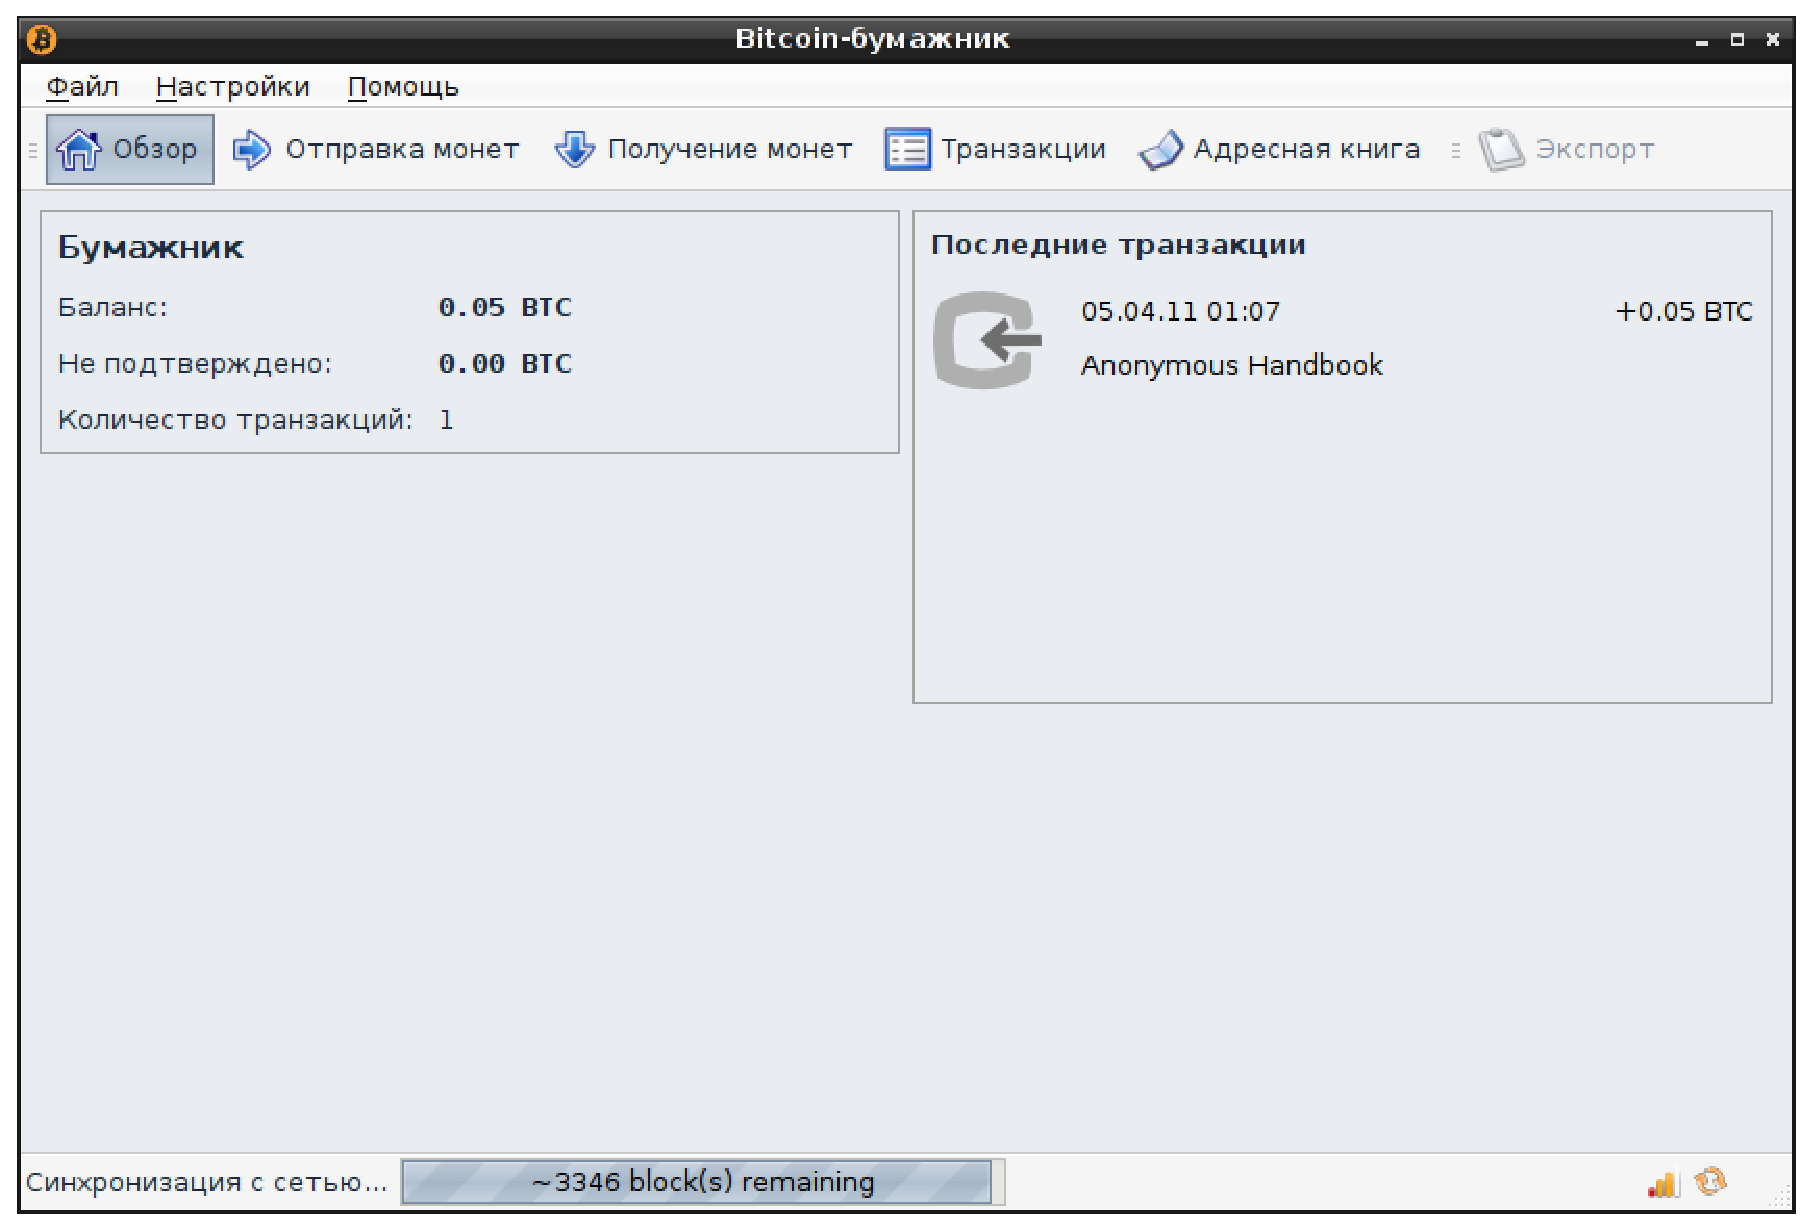
\includegraphics[width=0.75\linewidth]{bitcoin-screen}}
\caption{Интерфейс Bitcoin}
\end{figure}
При первом запуске Bitcoin автоматически создает кошелек. Адрес его можно увидеть на вкладке <<Получение монет>>. Там же вы можете создавать новые адреса, количество их не ограничено.
\subsubsection{Недостатки}
\begin{important}
Кошельки в Bitcoin анонимны, но все транзакции открыты и каждый может их просмотреть через сервисы, подобные \url{http://blockexplorer.com}. Проводите деньги через биржи.
\end{important}
\begin{enumerate}
\item Немгновенные транзакции.
\item Адреса кошельков сложно запомнить.
\item Так как у системы нет владельца, то ни заблокировать кошелек, попавший в руки мошенникам, ни вернуть вам деньги никто не сможет.
\end{enumerate}
\subsection{Liberty Reserve}
\textbf{Liberty Reserve} --- оффшорная платежная система, головной офис которой расположен в Сан-Хосе, Коста-Рика. Позволяет иметь кошельки в долларах США, евро и граммах золота. Транзакции являются неотменяемыми, данные, указываемые при регистрации, никем не проверяются. Комиссия составляет 1 \% от суммы транзакции, но не меньше 1 цента и не больше 3 долларов, снимается с получателя платежа.
\subsubsection{Регистрация}
Зайдите на сайт \url{https://www.libertyreserve.com/} и кликните на <<Create Account>>. Заполните форму. Не указывайте реальных данных. <<First Name>> --- имя, <<Last Name>> --- фамилия, <<Account Name>> --- логин, <<E-mail>> --- электронная почта, <<Re-enter e-mail>> --- повторить электронную почту, <<Security Question>> --- секретный вопрос, <<Answer>> --- ответ, <<Personal welcome message>> --- сообщение приветствия, <<Account Functions>> --- включить или не включать API, для большинства пользователей можно оставить <<User (API disabled)>> (не включать). Введите каптчу и кликайте <<Agree>> (принять).\\
На следующей странице для вас будет сгенерирован <<Password>> (пароль), <<Login PIN>> (PIN-код) и <<Master Key>> (мастер-ключ), также будут показан секретный вопрос и ответ на него, которые вы выбрали в предыдущей форме. Сохраните эти данные в безопасном месте. На почту вам должно придти письмо, в котором содержится ваш <<Liberty Reserve account number>> (персональный номер учетной записи). Его тоже необходимо сохранить в безопасном месте.\\
После этого вам нужно войти в свой аккаунт. Кликните на <<Login>> (вход) на сайте Liberty Reserve и введите свой <<Account Number>> из почты, пароль и каптчу. Нажмите <<Next>> (далее).\\
Будет показано сообщение приветствия (personal welcome message). Если оно совпадает с тем, которое вы вводили в момент регистрации, то значит вы находитесь на настоящем сайте Liberty Reserve, а не на фишинговой странице. Поставьте галочку на <<I confirm that my custom welcome message is correct>> (Я подтверждаю, что мое сообщение приветствия верно) и кликните <<Continue>> (продолжить).\\
Кликните на <<Login PIN>> и введите свой пин-код, выданый вам системой. Ввести его нужно с появившейся экранной клавиатуры. Нажмите <<Login>>.\\
Заполните форму, опять выдуманными данными. <<Address>> --- адрес, <<City>> --- город, <<Country>> --- страна, <<State/Region>> --- штат/регион, <<Zip/Postal Code>> --- почтовый индекс, <<Date of Birth>> --- дата рождения в формате мм/дд/гггг, <<Phone>> --- телефон, <<Account will be used for>> --- аккаунт будет использован для, <<Your Occupation>> --- род занятий. Нажмите на <<Submit>>.
\begin{enumerate}
\item 
\end{enumerate}

\section{IM-сервисы}
\subsection{I2P-Messenger}
\textbf{I2P-Messenger} --- программа мгновенного обмена сообщениями, работающая в сети I2P. Сайт: \url{http://echelon.i2p/qti2pmessenger}.
\subsection{TorChat}
\textbf{TorChat} --- программа мгновенного обмена сообщениями, работающая поверх Tor. Сайт: \url{https://github.com/prof7bit/TorChat}.
\subsection{JTorChat}
\textbf{JTorChat} --- версия TorChat, переписанная на Java. Сайт: \url{https://github.com/jtorchat/jtorchat}
\subsection{Cryptocat}
\textbf{Cryptocat} --- доступный через браузер чат-сервис с прозрачным шифрованием на Javascript. Сайт: \url{https://crypto.cat}.

\section{Ремейлеры}
\textbf{Ремейлеры} --- сервера, занимающиеся пересылкой сообщений электронной почты по указанному адресу.\\
Ремейлеры бывают псевдонимными (иногда их называют Type 0 или nym) и анонимными. Анонимные делятся на три типа:
\begin{enumerate}
\item Ремейлеры шифропанков
\item Mixmaster 
\item Mixminion
\end{enumerate}
\subsection{Ремейлеры шифропанков}
\textbf{Ремейлеры шифропанков (Type I)} --- ремейлеры, удаляющие из получаемых писем всю информацию, которая может быть использована для идентификации, и пересылающие их на указанный адрес. Зачастую письма можно посылать зашифрованными с помощью GPG. Возможно использование цепочек из нескольких ремейлеров.
\subsection{Mixmaster}
\textbf{Mixmaster (Type II)} --- ремейлеры, требующие установки специальной программы для отправки сообщений. Более безопасны, чем Type I, так как, например, пакеты с сообщениями всегда фиксированного размера, что не позволяет отслеживать письма по размеру. Сайт: \url{http://mixmaster.sourceforge.net}.
\subsection{Mixminion}
\textbf{Mixminion (Type III)} --- ремейлеры, также требующие установки специальной программы, но еще более безопасные, так как используют луковичную маршрутизацию и имеют еще несколько улучшений. Сайт: \url{http://mixminion.net}.

\section{Прием почты}
\begin{important}
Хозяева всех перечисленных сервисов (кроме I2P-Bote) могут читать вашу почту. Шифруйте отправляемые письма.
\end{important}
\subsection{I2P-Mail}
\textbf{I2P-Mail} --- обычный почтовый сервис, находящийся в сети I2P. Позволяет получить почту в домене mail.i2p и i2pmail.org. Пользоваться можно как внутри I2P, так и во внешнем интернете. Адрес: \url{http://hq.postman.i2p}.
\subsection{I2P-Bote}
\textbf{I2P-Bote} --- несовместимая с обычной почтой безсерверная анонимная почта, реализованая в виде плагина для I2P. Сайт: \url{http://i2pbote.i2p}, \url{http://i2pbote.net}.
\subsection{TorMail}
\textbf{TorMail} --- обычный почтовый сервис, работающий как скрытый сервис Tor. Позволяет получить почту в домене tormail.org. Ранее был доступен tormail.net, но он был зарегистрирован через русского регистратора RU-CENTER (nic.ru), который требовал предъявления документов, удостоверяющих личность\cite{tormail}. Адрес: \url{http://jhiwjjlqpyawmpjx.onion}.
\subsection{Privacybox}
\textbf{Privacybox} --- сервис анонимных контактых форм, работающий в I2P, Tor и обычном интернете. Адреса: \url{https://privacybox.de}, \url{http://privacybox.i2p}, \url{http://c4wcxidkfhvmzhw6.onion}.
\subsection{TorPM}
\textbf{TorPM} --- сервис обмена сообщениями, работающий через веб-сайт. Позволяет обмениваться простыми текстовыми сообщениями, напоминающими обычную электронную почту. Адрес: \url{http://4eiruntyxxbgfv7o.onion/pm}.

\section{Шифрование данных}
\subsection{Truecrypt}
\textbf{Truecrypt} --- кроссплатформенное приложение для шифрования данных на лету. Позволяет шифровать как запоминающие устройства, так и создавать контейнеры для хранения шифрованных данных. Имеет возможность создания скрытых томов --- к одному контейнеру можно получить доступ с помощью двух ключей, один из которых вы можете назвать, если к вам будет применено насилие, не раскрыв при этом содержимого секретного тома.
\subsubsection{Установка}
Для установки посетите \url{http://truecrypt.org} или установите пакет с помощью пакетного менеджера вашего дистрибутива.
\subsubsection{Использование}
\subsubsection{Недостатки}
\subsection{dm-crypt}
\textbf{dm-crypt} --- подсистема прозрачного шифрования в Linux и DragonFly BSD. Позволяет шифровать на лету блочные устройства. В Windows доступ к шифрованным dm-crypt данным можно получить с помощью FreeOTFE (\url{http://freeotfe.org}).
\subsubsection{Установка}
Хоть dm-crypt и является частью ядра и его использование возможно без установки дополнительных утилит, все же для удобства лучше установить пакеты cryptsetup (\url{https://code.google.com/p/cryptsetup}) и cryptmount (\url{http://cryptmount.sourceforge.net}).
\subsubsection{Использование}
\subsubsection{Недостатки}
\subsection{eCryptfs}
\subsubsection{Использование}
\subsubsection{Недостатки}
\subsection{GPG}
\subsubsection{Установка}
Для установки посетите \url{http://gnupg.org} или установите пакет с помощью пакетного менеджера вашего дистрибутива.
\subsubsection{Использование}
\subsubsection{Недостатки}

\section{Шифрование в IM}
\subsection{Off-the-Record Messaging (OTR)}
\begin{important}
OTR не подходит для шифрования офлайн-собщений, так как подтвержденный вам ключ используется только для передачи других ключей, генерируемых каждую сессию. Ключи, используемые для шифрования сообщений, удаляются после завершения сессии. Сделано это было для того, чтобы нельзя было доказать авторство сообщений после завершения диалога.
\end{important}
\textbf{OTR} --- криптографический протокол, предоставляющий шифрование в системах мгновенного обмена сообщениями. Встроенную поддержку имеют клиенты Adium, climm, MCabber, CenterIM, Phoenix Viewer, Vacuum IM, Jitsi, BitlBee, Spark, с помощью плагина OTR доступен в Pidgin\cite{otr-pidgin}, Kopete\cite{otr-kopete}, Miranda IM\cite{otr-miranda}, Psi+\cite{otr-psi}, Trillian\cite{otr-trillian}, irssi\cite{otr-irssi}, Gajim\cite{otr-gajim}. Также существует OTR localhost AIM Proxy, позволяющая использовать OTR в любом клиенте, но на данный момент поддерживаются только протоколы AIM/ICQ. Сайт: \url{http://cypherpunks.ca/otr/}, плагины для вашего клиента предоставляются сторонними разработчиками.
\subsection{GPG и Jabber}
\textbf{XEP-0027} --- расширение протокола XMPP (Jabber), позволяющее использовать GPG (OpenPGP) для шифрования сообщений\cite{xep-0027}. Поддерживается клиентами Centericq, Gajim, Kopete, Psi и Miranda IM (с помощью плагина).

\section{Шифрование почты}
\subsection{GPG}
GPG позволяет шифровать любые данные, в том числе и почтовые сообщения. Подробнее работа GPG рассматривается в разделе <<Шифрование данных>>.
\subsubsection{Enigmail}
Enigmail --- дополнение для почтового клиента Thunderbird и набора приложений SeaMonkey, предоставляющее удобный интерфейс для работы c GPG в почтовых сообщениях. Сайт: \url{http://enigmail.net}.
\subsection{S/MIME}
\textbf{S/MIME} (\textbf{Secure/Multipurpose Internet Mail Extensions}) --- стандарт подписи и шифрования электронной почты.
\subsubsection{Получение бесплатного сертификата}
Бесплатно сертификат можно получить у следующих центров сертификации:
\begin{enumerate}
\item \url{https://cert.startcom.org}
\item \url{https://secure.comodo.com/products/frontpage?area=SecureEmailCertificate}
\item \url{https://www.cacert.org/index.php?id=1} (корневой сертификат присутствует не везде)
\end{enumerate}
\subsubsection{Создание самоподписанного сертификата}
Для этого нам понадобится OpenSSL (\url{https://openssl.org}).
\begin{lstlisting}
openssl genrsa -des3 -out server.key 1024
openssl req -new -key server.key -out server.csr
openssl x509 -req -days 365 -in server.csr -signkey server.key -out server.crt
\end{lstlisting}
\subsubsection{Использование}
Для использования импортируйте ключ в ваш почтовый клиент. Сохраните ключи в безопасности.

\section{Стеганография}
\begin{important}
Использование стеганографии само по себе не делает недоступной передаваемую информацию, зная метод (что случается при использовании общедоступной программы) или подвергнув изображение стеганализу можно прочитать скрытую таким образом информацию. Используйте стеганографию совместно со сторонними или встроенными криптографическими утилитами.
\end{important}
\textbf{Стеганография} --- способ тайной передачи информации путем сохранения в тайне самого факта передачи информации. Чаще всего используется совместно с криптографическими методами.
\subsection{steghide}
\subsubsection{Установка}
Для установки посетите \url{http://steghide.sourceforge.net/} или установите пакет с помощью пакетного менеджера вашего дистрибутива.
\subsubsection{Использование}
\begin{figure}[ht!]
\vspace{-4ex}
\centering
\subfigure[]{
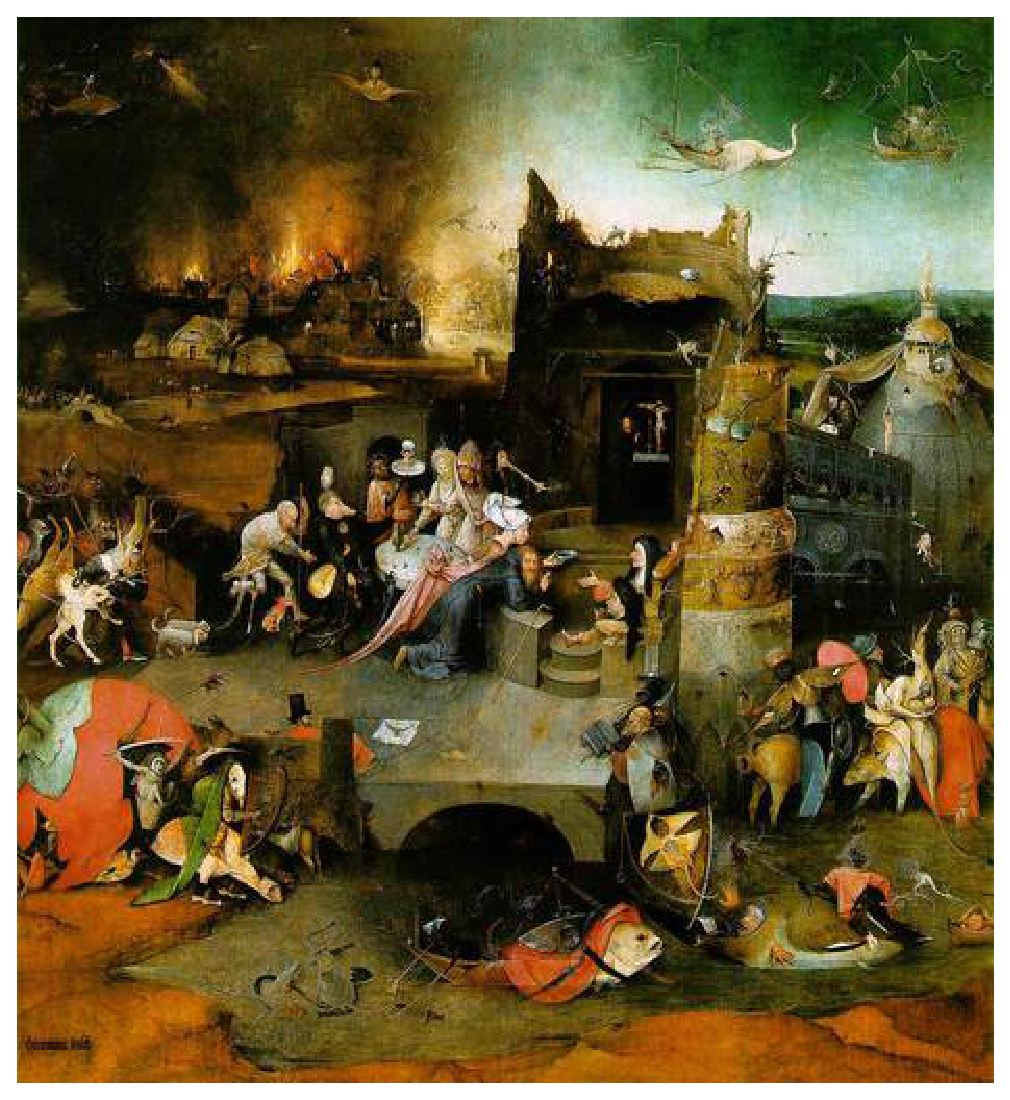
\includegraphics[width=0.25\linewidth]{original}
\label{fig:original}
}
\hspace{4ex}
\subfigure[]{
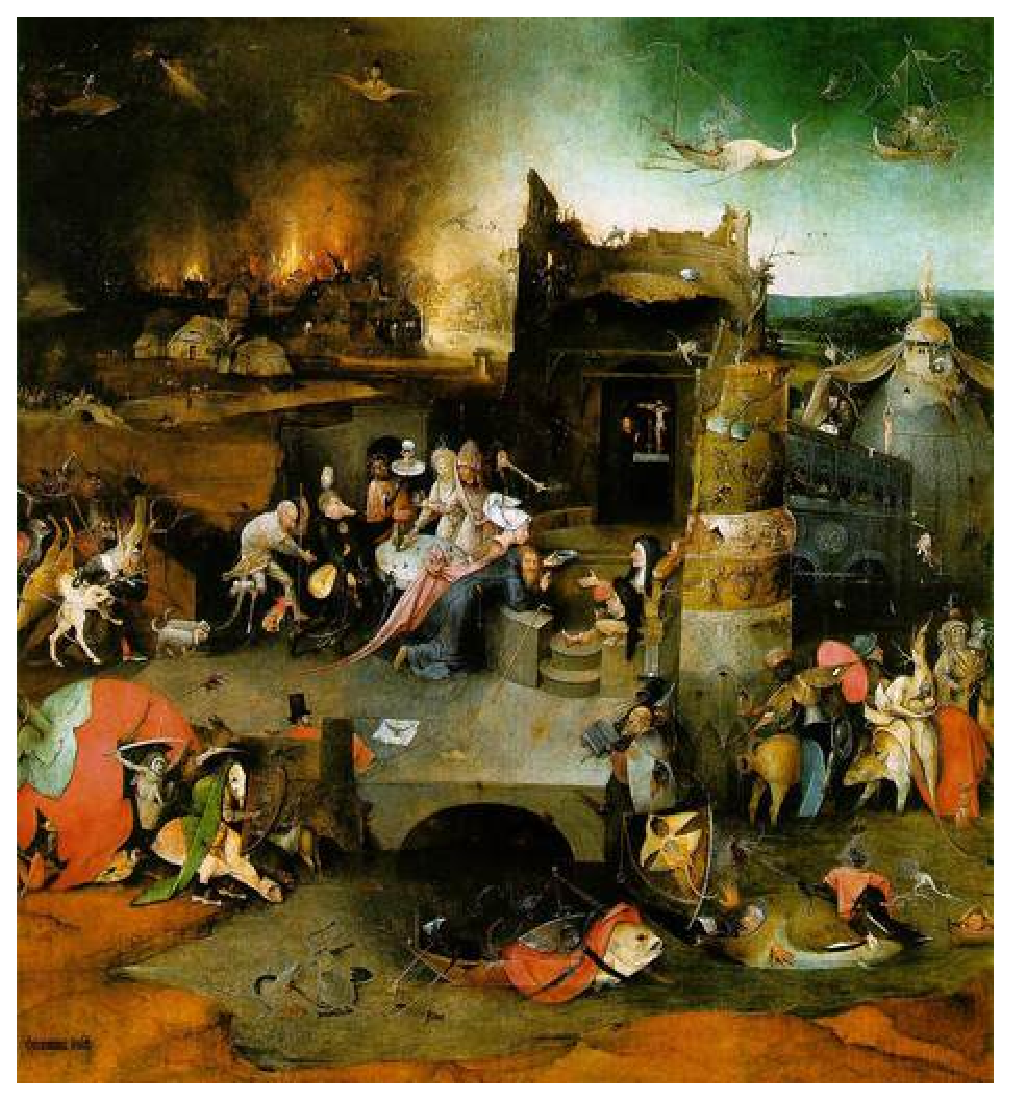
\includegraphics[width=0.25\linewidth]{steghide1}
\label{fig:steghide1}
}
\hspace{4ex}
\subfigure[]{
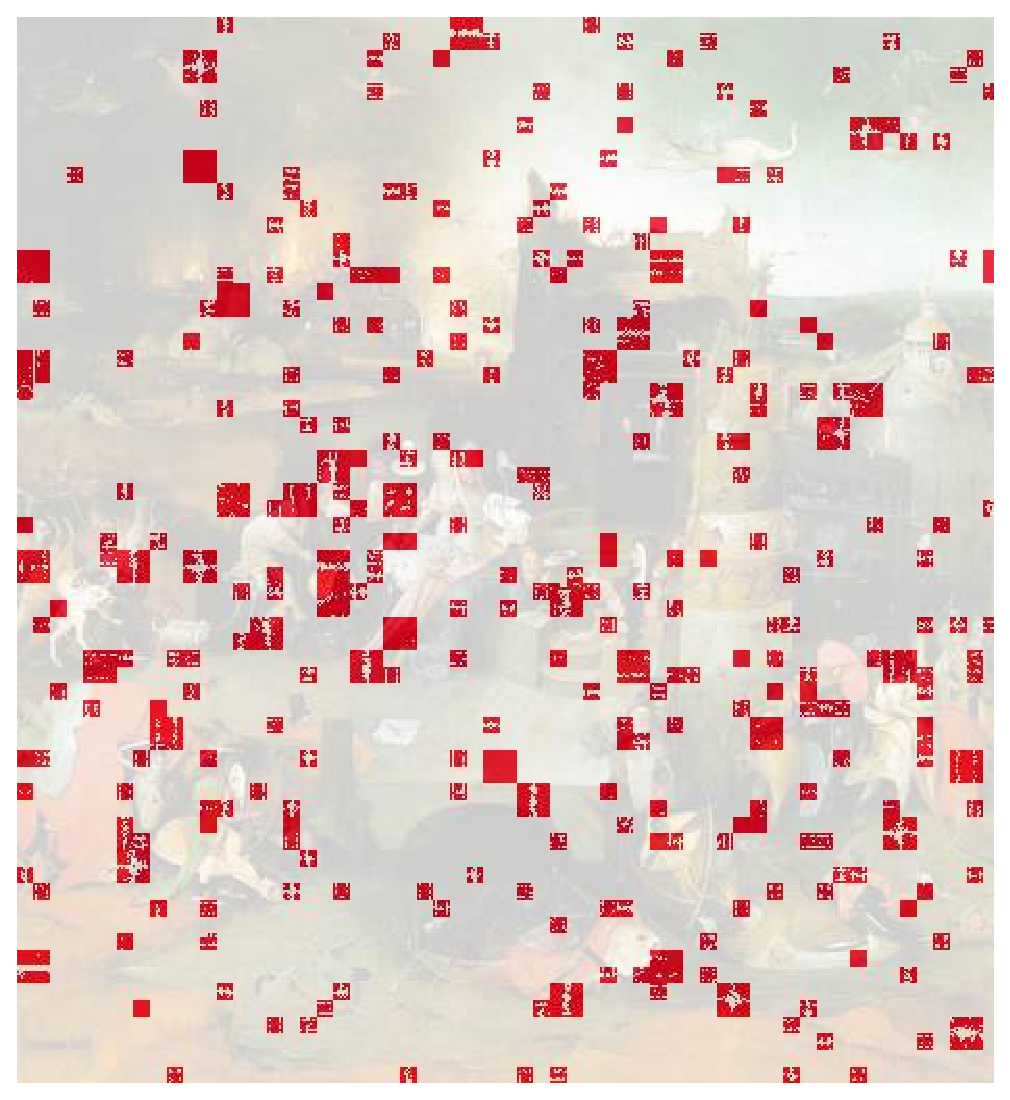
\includegraphics[width=0.25\linewidth]{steghide2}
\label{fig:steghide2}
}
\caption{Использование steghide: 
\subref{fig:original} исходное изображение; 
\subref{fig:steghide1} в изображении закодирована фраза <<Feci quod potui, faciant meliora potentes>> с паролем <<cogitoergosum>>; 
\subref{fig:steghide2}} разница между изображениями.
\end{figure}
Вставка данных в изображение:
\begin{lstlisting}
steghide embed -cf "coverfile.jpg" -ef "embedfile.txt" -sf "stegofile.jpg" -p "password"
\end{lstlisting}
coverfile.jpg --- файл, в который вставляются данные.\\
embedfile.txt --- файл, который вставляется в изображение.\\
stegofile.jpg --- файл со вставленным изображением.\\
password --- пароль.\\\\
Извлечение данных:
\begin{lstlisting}
steghide extract -sf "stegofile.jpg" -p "password" -xf "extractfile.txt"
\end{lstlisting}
stegofile.jpg --- файл со вставленным изображением.\\
password --- пароль.\\
extractfile.txt --- файл, в который нужно записать извлеченные данные.
\subsubsection{Недостатки}
\subsection{OpenStego}
\subsubsection{Установка}
Для установки посетите \url{http://openstego.sourceforge.net/} или установите пакет с помощью пакетного менеджера вашего дистрибутива.
\subsubsection{Использование}
\begin{figure}[h]
\center{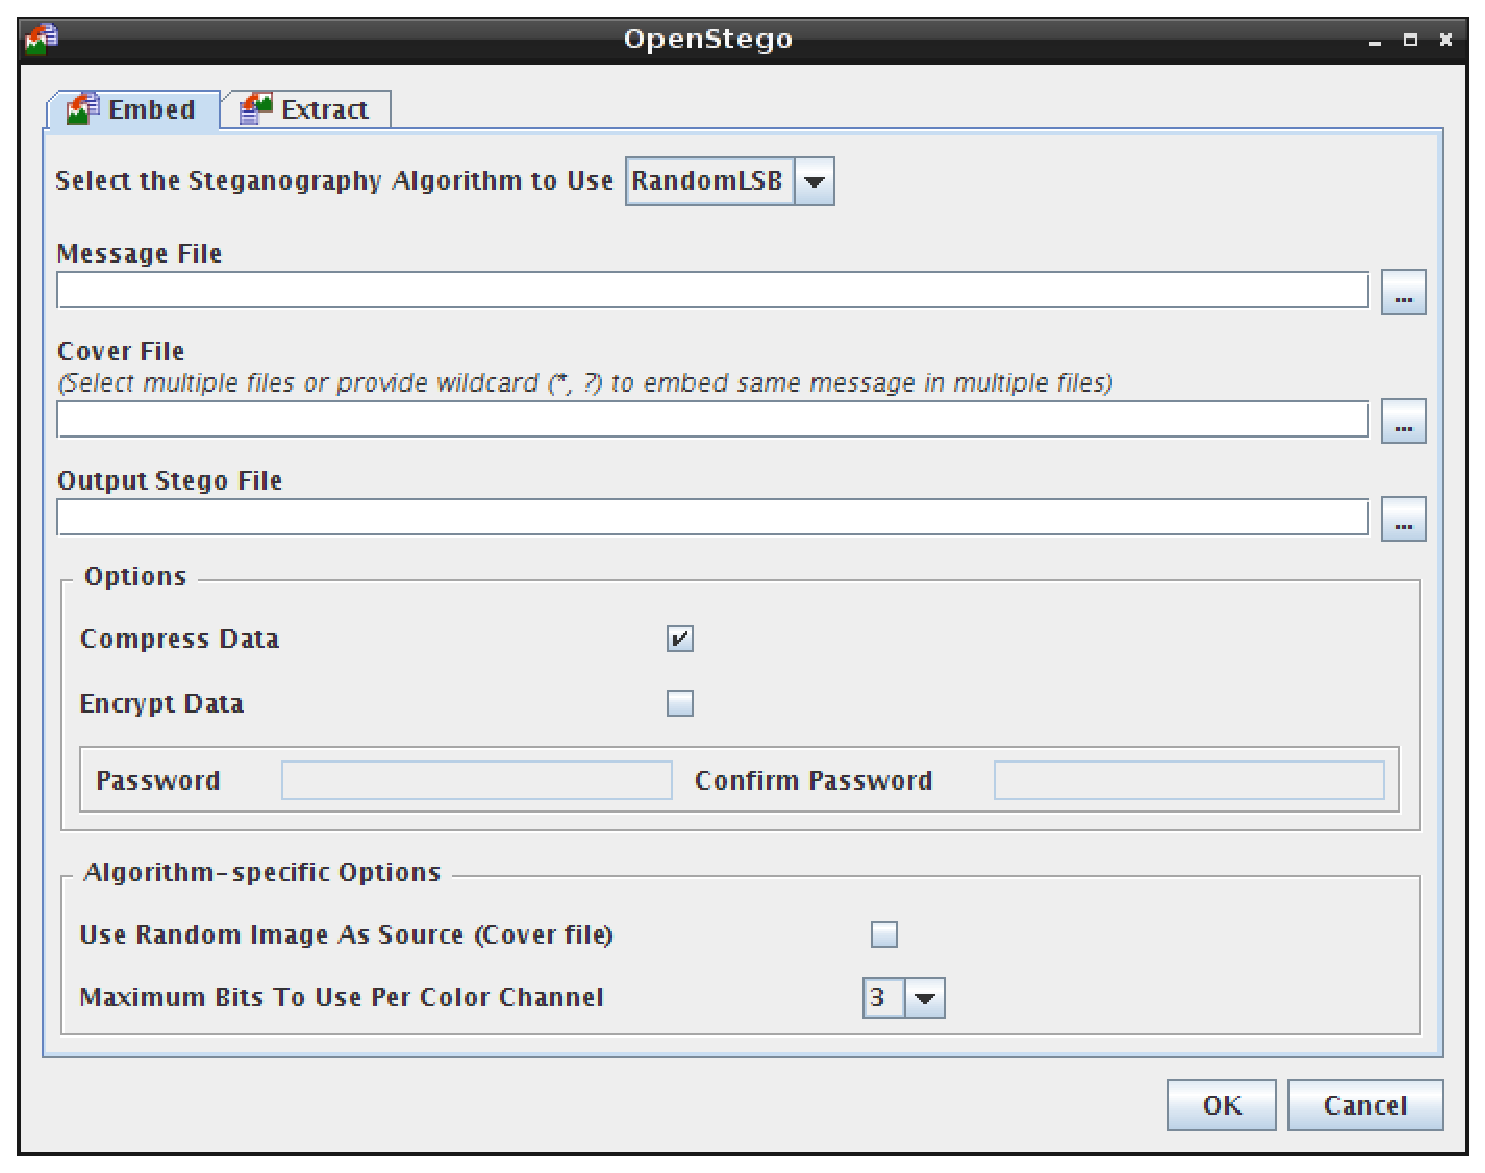
\includegraphics[width=0.75\linewidth]{openstego}}
\caption{Интерфейс OpenStego}
\end{figure}
\begin{figure}[ht!]
\vspace{-4ex}
\centering
\subfigure[]{
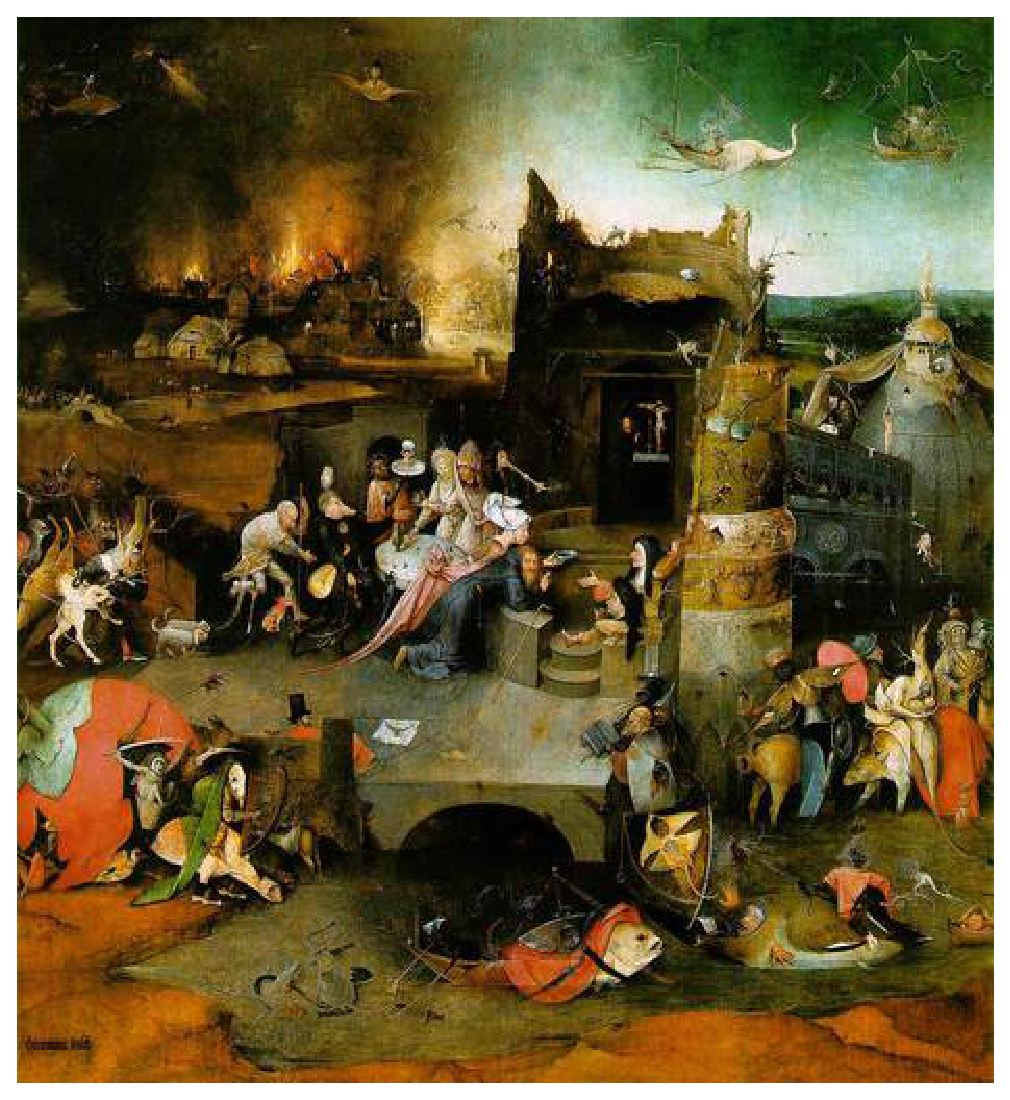
\includegraphics[width=0.25\linewidth]{original}
\label{fig:original}
}
\hspace{4ex}
\subfigure[]{
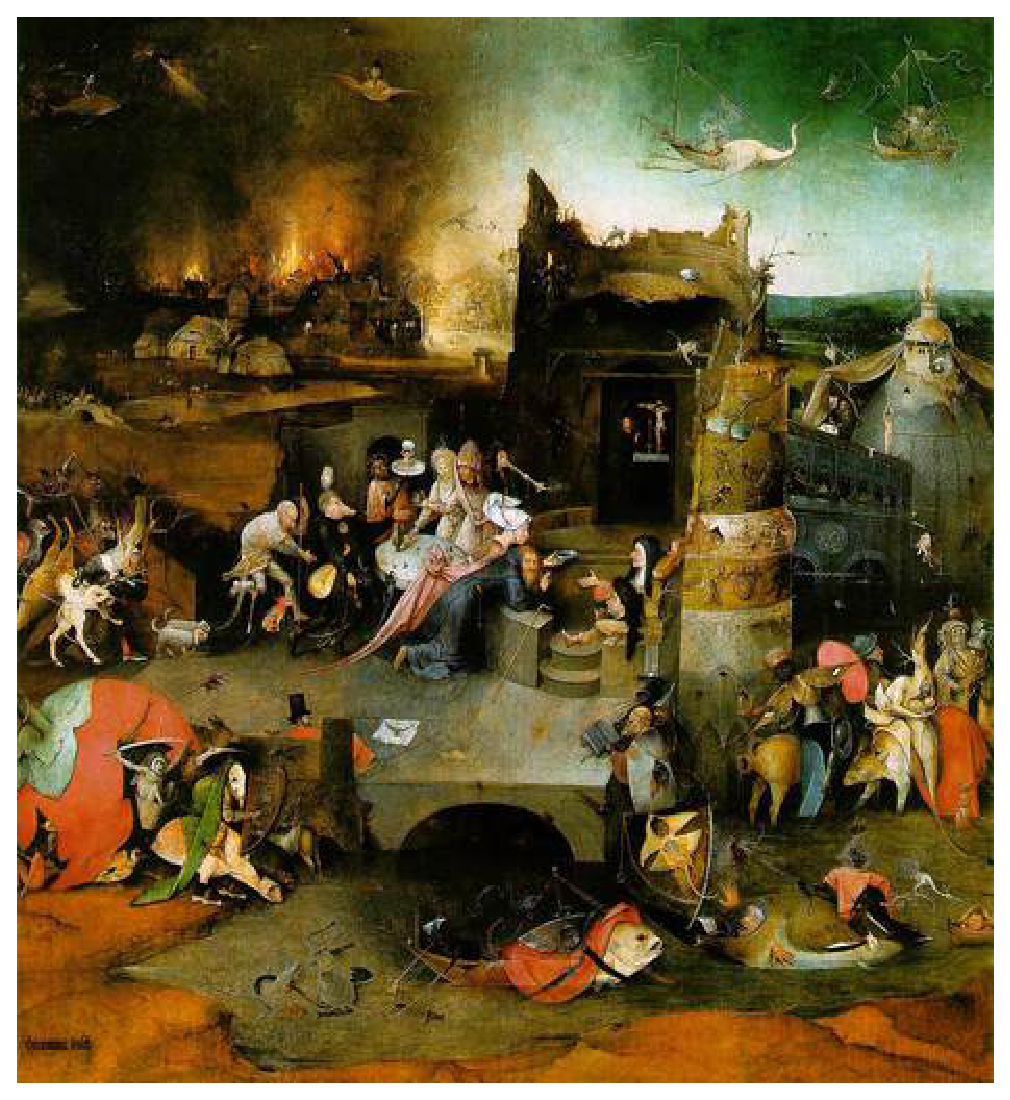
\includegraphics[width=0.25\linewidth]{openstego1}
\label{fig:openstego1}
}
\hspace{4ex}
\subfigure[]{

\includegraphics[width=0.25\linewidth]{openstego2}
\label{fig:openstego2}
}
\caption{Использование OpenStego:
\subref{fig:original} исходное изображение;
\subref{fig:openstego1} в изображении закодирована фраза <<Feci quod potui, faciant meliora potentes>> без пароля;
\subref{fig:openstego2}} разница между изображениями.
\end{figure}
\subsubsection{Недостатки}
\subsection{StegoShare}
StegoShare специально приспособлен для того, чтобы прятать несколько файлов в нескольких изображениях и расшаривать их в P2P-сетях.
\subsubsection{Установка}
Для установки посетите \url{http://stegoshare.sourceforge.net} или установите пакет с помощью пакетного менеджера вашего дистрибутива.
\subsubsection{Использование}
\begin{figure}[h]
\center{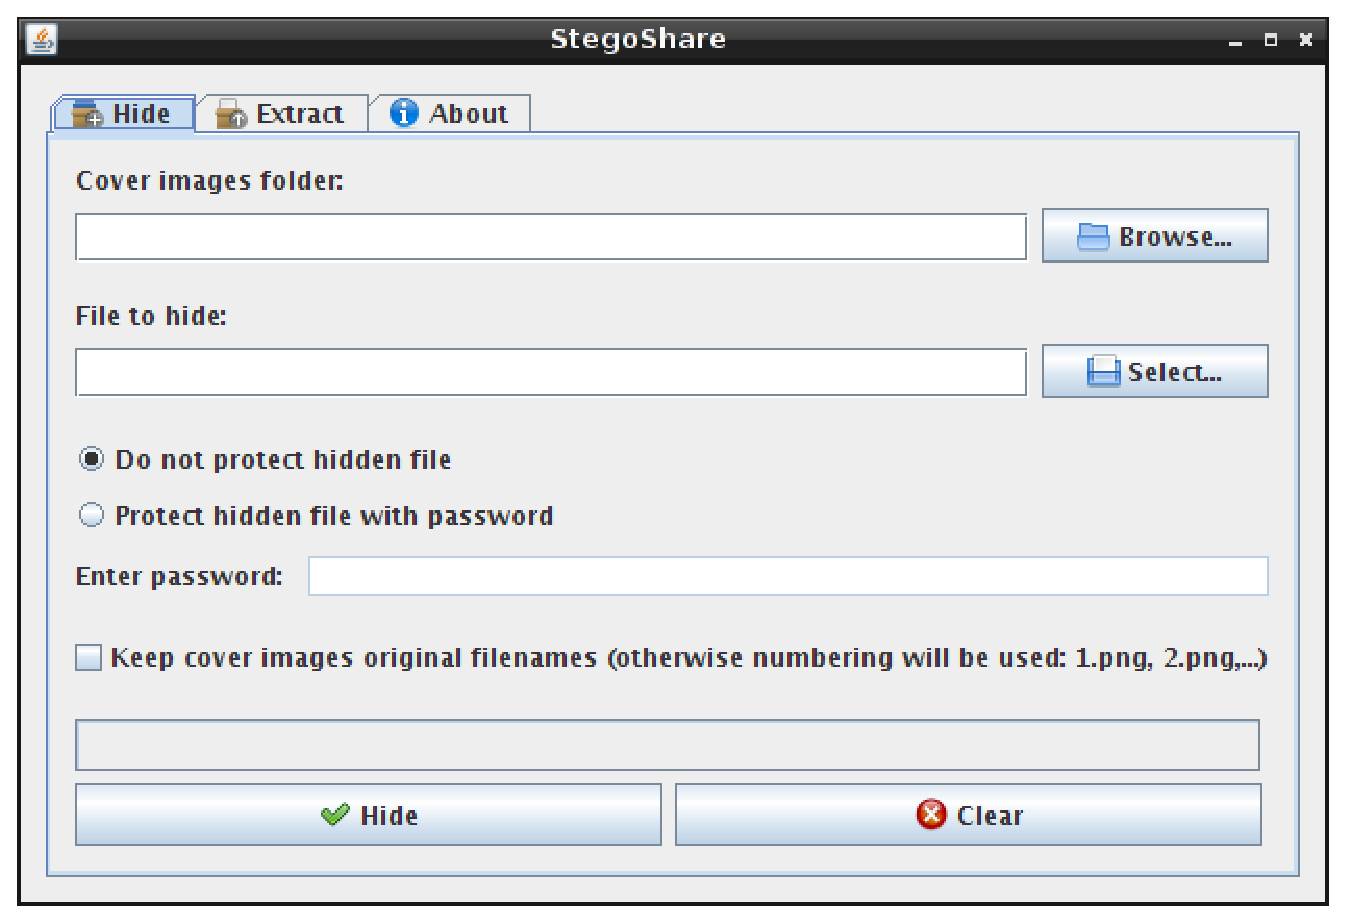
\includegraphics[width=0.75\linewidth]{stegoshare}}
\caption{Интерфейс StegoShare}
\end{figure}
\begin{figure}[ht!]
\vspace{-4ex}
\centering
\subfigure[]{
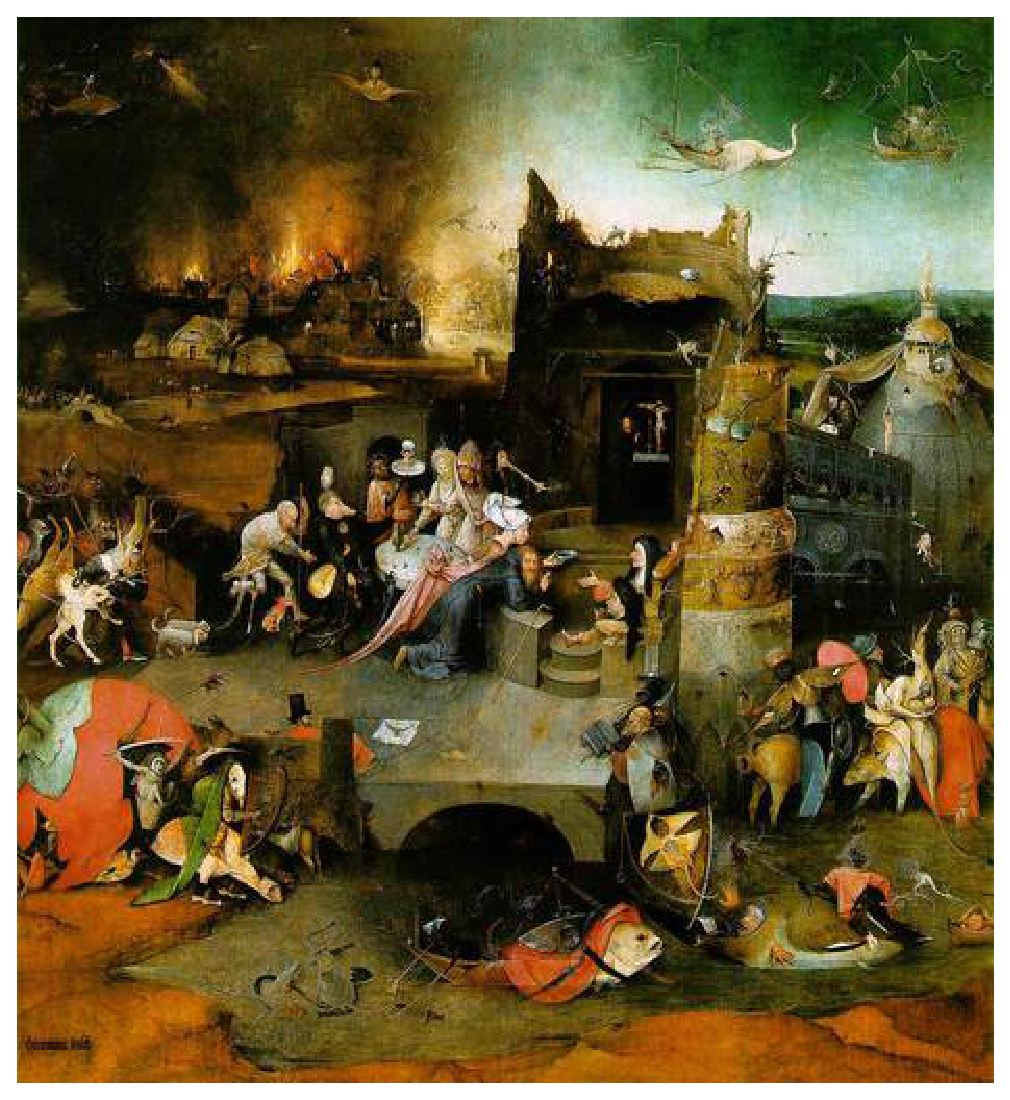
\includegraphics[width=0.25\linewidth]{original}
\label{fig:original}
}
\hspace{4ex}
\subfigure[]{
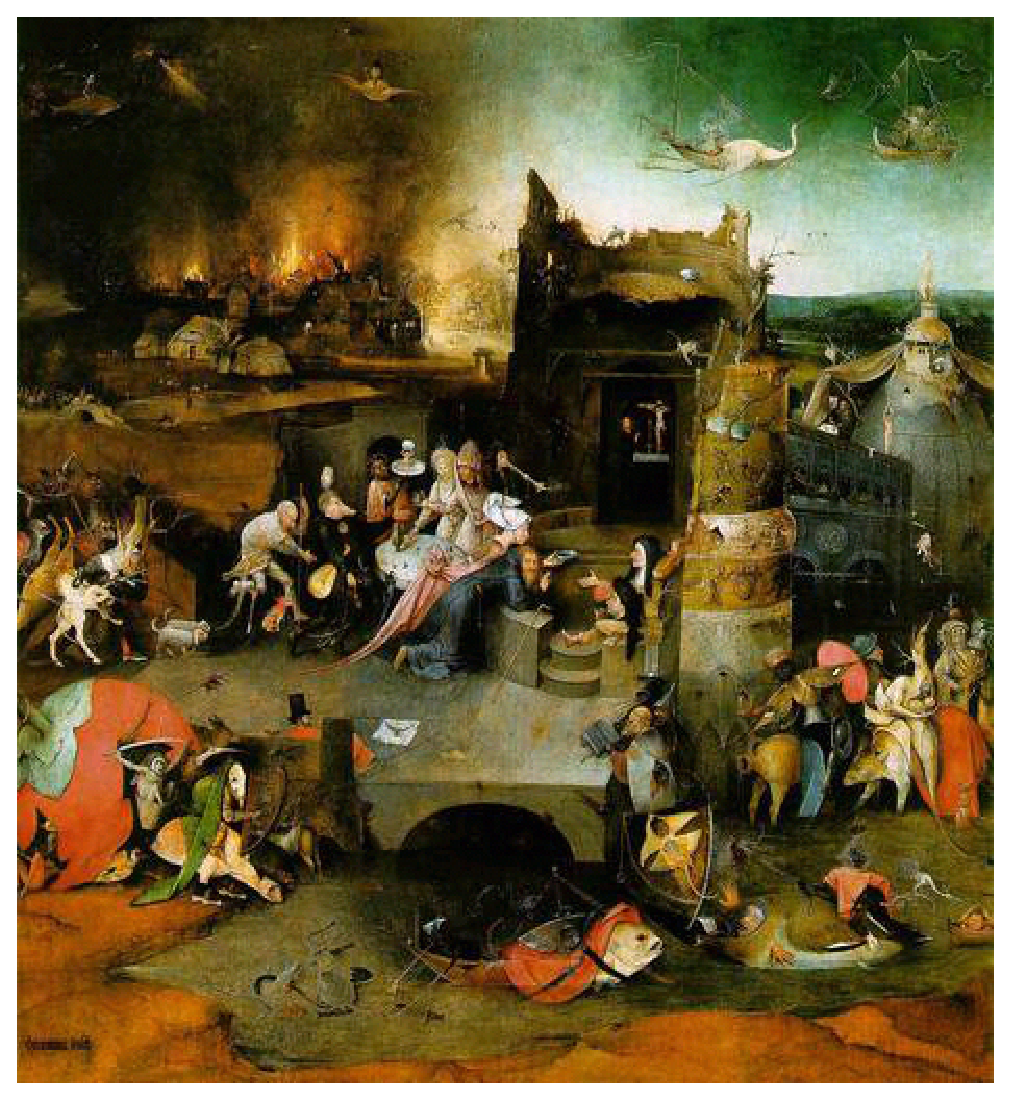
\includegraphics[width=0.25\linewidth]{stegoshare1}
\label{fig:stegoshare1}
}
\hspace{4ex}
\subfigure[]{

\includegraphics[width=0.25\linewidth]{stegoshare2}
\label{fig:stegoshare2}
}
\caption{Использование StegoShare:
\subref{fig:original} исходное изображение;
\subref{fig:stegoshare1} в изображении закодирована фраза <<Feci quod potui, faciant meliora potentes>> без пароля;
\subref{fig:stegoshare2}} разница между изображениями.
\end{figure}
\subsubsection{Недостатки}

\subsection{Желтые точки}
\begin{wrapfigure}[9]{r}{0.25\linewidth}
\includegraphics[width=\linewidth]{dots}
\caption{Желтые точки. Изображение: Parhamr}
\end{wrapfigure}
При печати материалов (например, листовок) не стоит забывать, что многие принтеры кодируют микроточками информацию о времени печати и о серийном номере принтера \cite{eff_dots}. Данная информация может быть использована для установления личности авторов отпечатков. Список принтеров, размещающих и не размещающих желтые точки смотрите в отчете Electronic Frontier Foundation\cite{eff_list}.

\section{Альтернативные DNS}
\subsection{Namecoin}
\textbf{Namecoin} --- распределенная система доменных имен, основанная на Bitcoin, хранящая в блоках информацию о доменах. Она сохранила многие плюсы Bitcoin, например, никто не может заблокировать ни один домен. В настоящее время возможно получение доменов в зоне .bit, однако воспользоваться ими смогут только те, кто предварительно настроил свой компьютер.
\subsubsection{Установка}
\begin{important}
Стоит заменить, что все методы, не подразумевающие установку собственного резолвера, не безопасны. При использовании прокси-серверов владелец может перехватывать все данные, а при использовании открытых DNS-серверов владелец может установить сам факт посещения конкретного сайта.
\end{important}
Существует несколько способов использовать Namecoin.
\begin{enumerate}
\item Использовать открытый прокси, адреса которых перечислены здесь \url{https://dot-bit.org/How_To_Browse_Bit_Domains#List_of_App_proxies}.
\item Использовать альтернативный DNS-сервер с поддержкой Namecoin, адреса открытых серверов перечислены здесь \url{https://dot-bit.org/How_To_Browse_Bit_Domains#List_of_DNS_servers}.
\item Использовать DNS-суффикс \url{https://dot-bit.org/How_To_Browse_Bit_Domains#List_of_DNS_suffixes}.
\item Использовать веб-прокси \url{https://dot-bit.org/How_To_Browse_Bit_Domains#List_of_Web_proxies}.
\item Использовать BIND с NamecoinToBind.\\Подробнее \url{https://github.com/khalahan/NamecoinToBind}.
\item Использовать ncproxy совместно с Tor (наилучший вариант): \url{https://dot-bit.org/forum/viewtopic.php?p=1448#p1448}.
\item Использовать NmcSocks (тоже возможно использование вместе с Tor): \url{https://github.com/itsnotlupus/nmcsocks}.
\end{enumerate}
\subsubsection{Недостатки}
\subsection{OpenNIC}
\subsection{Собственный кеширующий DNS сервер}

\section{Хранение паролей}
\begin{important}
Не используйте один и тот же пароль на нескольких ресурсах и не используйте простых паролей. Не храните пароли в открытом виде, пользуйтесь менеджерами паролей, которые используют криптографические методы для предотвращения кражи ваших паролей.
\end{important}
\subsection{KeePassX}
\textbf{KeePassX} (не путать с KeePass) --- кроссплатформенный менеджер паролей, распространяющийся на условиях GNU GPL v2, форк KeePass. Сайт: \url{https://keepassx.org}.
\subsection{KeePass}
\textbf{KeePass} --- кроссплатформенный (через Mono) менеджер паролей. Сайт: \url{http://keepass.info}.
\subsection{KWallet}
\textbf{KWallet} --- кроссплатфоменный менеджер паролей, разрабатывающийся в рамках проекта KDE. Сайт: \url{http://utils.kde.org/projects/kwalletmanager/}.
\subsection{Revelation}
\textbf{Revelation} --- менеджер паролей для GNU/Linux и *BSD. Сайт: \url{http://revelation.olasagasti.info}.

\section{Безопасное удаление файлов}
\begin{important}
Простое удаление файлов оставляет возможность для восстановления, так как файлы на самом деле никуда не исчезают, а просто помечаются как удаленные и на этот сектор диска становится возможна запись.
\end{important}
\subsection{shred}
\textbf{shred} --- утилита из пакета GNU coreutils, позволяющая переписывать указанные файлы несколько раз, что делает практически невозможным их восстановление. Сайт GNU coreutils: \url{http://www.gnu.org/software/coreutils}.
\subsubsection{Использование}
\begin{lstlisting}
shred -u "файл"
\end{lstlisting}
\subsubsection{shreg}
shreg --- графический интерфейс для shred. Сайт: \url{https://github.com/arxell/shreg}.
\subsection{wipe}
\textbf{wipe} --- аналогичная утилита для UNIX-подобных систем, работающая по тому же принципу. Сайт: \url{http://lambda-diode.com/software/wipe/}.
\subsubsection{Использование}
\begin{lstlisting}
wipe "файл"
\end{lstlisting}
\section{Метаданные}
\begin{important}
В метаданных может храниться огромное количество информации о создателе файла.
\end{important}
\subsection{mat}
\textbf{mat} --- утилита, позволяющая удалять метаданные из файлов png, jpg, Open Document Format (.odt, .odx, .ods, ...), MS Office OpenXML (.docx, .pptx, .xlsx, ...), pdf, tar, zip, mp3, mp2, mp1, mpa, ogg, flac, torrent. Сайт: \url{https://mat.boum.org}.
\subsubsection{Использование}
\begin{lstlisting}
mat "файл"
\end{lstlisting}
